% =============================================================================================
\section{Backspin against the no-spin twin over the whole field}
\label{sec:svt}

Section~\ref{sec:field-chance} compared the best backspin setting with the no-spin twin at one spot. This
section repeats that comparison at every legal pose of a coarse field grid (code \code{src/spin\_vs\_twin.py},
data \code{data/spin\_vs\_twin.csv}, notes \code{research/SPIN\_VS\_TWIN.md}). Every chance is a model
probability\predicted{} under ASSUMED launch scatter and ASSUMED air sets. It is not a hit rate. The twin is
a yardstick, not a design. The one-wheel hood always spins the ball: $S$ runs from $1.029$\predicted{} to
$1.274$\predicted{} over the parameter box of Section~\ref{sec:launcher:Sband}, and falls below $1$ only with
a fast feeder. A shooter without spin would be a different mechanism. ``Twin $>$ spin'' therefore means that
backspin gives no gain in this model, not that a no-spin shooter should be built.

% ---------------------------------------------------------------------------------------------
\subsection{Grid, searches and verdict}
\label{sec:svt-method}

\paragraph{Grid.} The release points are $x\in\{\pm0.65,\pm0.95,\pm1.25,\pm1.55\}$\,\unit{m}\assumed{} in the
field frame of Section~\ref{sec:field-oblique} ($x<0$ is the far, unfavourable side; $x>0$ the near,
favourable side) and $y$ from
$-1.2$\assumed{} to $2.0$\,\unit{m}\assumed{} in steps of $0.4$\,\unit{m}\assumed. The release heights are
$h\in\{0.35,\,0.5,\,0.737\}$\,\unit{m}\assumed{} and the backspin values $S\in\{0.5,\,1.0,\,1.5\}$\assumed.
Of the $216$\derived{} poses $(x,y,h)$, $144$\derived{} are scored: $84$\derived{} on the unfavourable side
and $60$\derived{} on the favourable side. Of the other $72$\derived, $48$\derived{} put the
$0.457$\,\unit{m}\confirmed{} robot into a wall or the A-frame base, $15$\derived{} have a bearing $\psi$
(Eq.~\eqref{eq:field-psi}) above $60^\circ$\assumed{}, which the model flags as extrapolated, and
$9$\derived{} lie outside the exported tables.

\paragraph{Searches.} At each pose, three kinds of search run the best-chance procedure of
Section~\ref{sec:field-chance}. The candidates are clean settings inside the $8.9$\,\unit{m/s}\predicted{}
grip limit: up to $24$ grid settings, plus the tolerant lowest-rpm and lowest-hood settings and the most
forgiving one (Section~\ref{sec:field-solver}), $17$\derived{} to $27$\derived{} per search here. Each search
scores every candidate with $64$ shots, takes at most $5$ on to $400$ shots, and scores the winner on $1000$
fresh shots (seed $20261031$, common random numbers).
\begin{itemize}
  \item \textbf{Twin:} $S=0$, no lift, on its own clean grid.
  \item \textbf{Robust}$(S)$: one setting from the nominal set's clean grid, scored over the three lift sets
    pooled with equal weight\assumed{} and reported per set. This is the setting a team would pick without
    knowing the lift.
  \item \textbf{Tuned}$(S,L)$: the best setting for lift set $L$ alone, from that set's clean grid. This is
    the setting a team would pick after the lift has been measured.
\end{itemize}
The twin and every backspin winner at a pose are scored on the same fresh draws, so each pair is matched.

The lift sets are low, nominal and high from Table~\ref{tab:flight-clsets}. Every shot uses
$C_d=0.5$\assumed{} and $k=0.03$\,\unit{1/s}\assumed. The launch scatter is $1.5\,\%$\assumed{} in exit speed,
$0.40^\circ$\assumed{} in elevation and $0.50^\circ$\assumed{} in heading ($1\sigma$), with no spin scatter.
A shot counts only if it enters cleanly; bounce-ins are not scored.

\paragraph{Verdict.} Let $[\ell_s,u_s]$ and $[\ell_t,u_t]$ be the Wilson $95\,\%$ intervals
(Section~\ref{sec:robust_spec-wilson}) of the backspin and twin chances at one pose. Then
\begin{equation}
  \text{verdict}=\begin{cases}
    \text{spin} > \text{twin}, & \ell_s>u_t,\\
    \text{twin} > \text{spin}, & \ell_t>u_s,\\
    \text{unclear}, & \text{otherwise (the intervals overlap)}.
  \end{cases}
  \label{eq:svt-verdict}
\end{equation}
Near $p=0.35$\predicted{} with $n=1000$ the half-width of each interval is about $0.03$\derived, so a verdict
needs a gap of about $0.06$\derived. The matched difference is $\Delta p=p_s-p_t$ on the same draws.

% ---------------------------------------------------------------------------------------------
\subsection{Results}
\label{sec:svt-results}

Table~\ref{tab:svt-unfav} gives the unfavourable side at $S=1.0$, and Fig.~\ref{fig:svt} shows every pose
there. No row has the verdict spin $>$ twin: not on either side, nor for any $S$, search or lift set
($0$\predicted{} of $2592$\derived{} rows).

\begin{table}[htbp]
  \centering
  \caption{Unfavourable side, $84$\derived{} scored poses, $S=1.0$. The $S=1.5$ rows are identical
    (Section~\ref{sec:svt-sat}). The table gives the medians over the poses of the backspin and twin chances and
    of $\Delta p$, the verdict counts of Eq.~\eqref{eq:svt-verdict}, and the cost of not knowing the lift (tuned
    minus robust at the same pose, median $[\min,\max]$). All values are \predicted, in percent or percentage
    points (pp).}
  \label{tab:svt-unfav}
  \small
  \begin{tabular}{@{}llrrrrrl@{}}
    \toprule
    search & lift set & backspin (\%) & twin (\%) & $\Delta p$ (pp) & twin $>$ spin & unclear
      & tuned $-$ robust (pp) \\
    \midrule
    robust & low     & 16.0 & 35.2 & $-20.4$ & 84 & 0  & \\
    robust & nominal & 28.4 & 35.2 & $-8.1$  & 61 & 23 & \\
    robust & high    & 4.4  & 35.2 & $-31.4$ & 84 & 0  & \\
    \addlinespace
    tuned  & low     & 35.7 & 35.2 & $-0.3$  & 0  & 84 & $20.1$ $[14.3,\,28.4]$ \\
    tuned  & nominal & 35.3 & 35.2 & $-0.5$  & 0  & 84 & $7.3$ $[0.0,\,14.4]$ \\
    tuned  & high    & 34.4 & 35.2 & $-1.0$  & 0  & 84 & $30.1$ $[21.7,\,45.4]$ \\
    \bottomrule
  \end{tabular}
\end{table}

\begin{figure}[tbp]
  \centering
  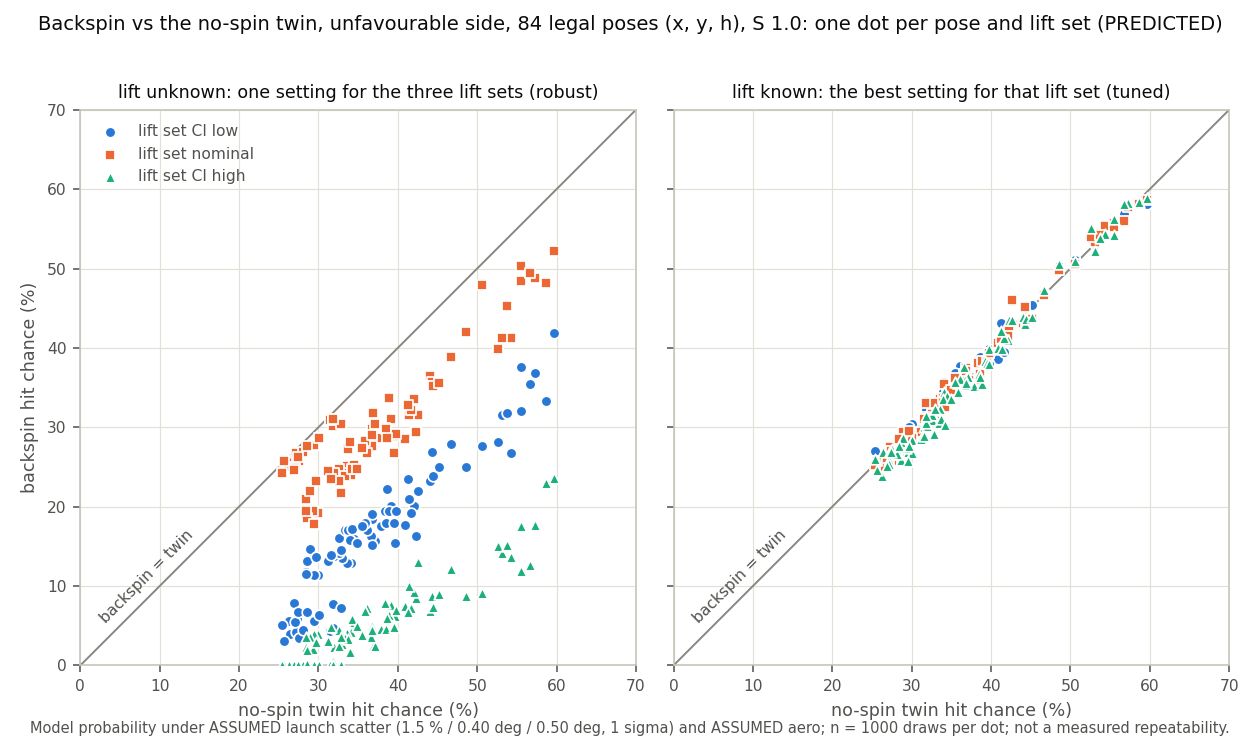
\includegraphics[width=\linewidth]{spin_vs_twin.png}
  \caption{Backspin chance against the twin's chance at every scored unfavourable-side pose, $S=1.0$ (model
    output \predicted{} under ASSUMED scatter and air sets). Left: robust, one setting for all three lift sets
    (the lift unknown). Right: tuned, the setting for the true lift set. Colour and marker give the lift set. A
    dot on the diagonal means backspin $=$ twin. Data: \code{data/spin\_vs\_twin.csv}.}
  \label{fig:svt}
\end{figure}

\paragraph{Lift known: level with the twin.} Tuned backspin and the twin are level at all $84$\derived{}
unfavourable-side poses, for every lift set. The medians are $34.4$\predicted{} to $35.7\,\%$\predicted{}
against $35.2\,\%$\predicted. At $S=1.0$ the median $\Delta p$ is $-0.3$\predicted, $-0.5$\predicted{} and
$-1.0$\,pp\predicted{} for the low, nominal and high sets, with a full range of $-3.9$\predicted{} to
$+3.4$\,pp\predicted. Backspin is lower at $51$\predicted, $62$\predicted{} and $65$\predicted{} of the $84$
poses. All poses use the same seeded draws, so these counts are not independent tests. The lean is also much
smaller than the half-width of each interval, so the model does not resolve it.

\paragraph{Lift unknown: below the twin.} One setting for all three lift sets puts backspin clearly below the
twin at $84$\predicted, $61$\predicted{} and $84$\predicted{} of the $84$ poses. Robust backspin reaches
$50\,\%$ at $2$\predicted{} poses (nominal set only), the twin at $11$\predicted. This is the cost of not
knowing the lift, $7.3$\predicted{} to $30.1$\,pp\predicted{} at the median (last column of
Table~\ref{tab:svt-unfav}). It is not an advantage of a ball without spin. The robust search pools only the
lift uncertainty, the twin has no lift to pool, and $C_d$ has the same fixed value for both shots. If $C_d$ were
uncertain too, both shots would pay for it; that case was not run. Tuning on the real ball, or measuring its
lift, removes the cost in the model.

\paragraph{Favourable side.} Both shots enter almost always: medians $99.7$\predicted{} to
$99.8\,\%$\predicted{} against $99.8\,\%$\predicted. Every pose is unclear except $3$\predicted{} in robust
$S=0.5$ with the high set, where the twin is clearly higher ($97.9$\predicted{} to $98.6\,\%$\predicted{}
against $99.8$\predicted{} to $99.9\,\%$\predicted).

\paragraph{Where on the unfavourable side.} The twin's chance ranges from $25.4$\predicted{} to
$59.7\,\%$\predicted{} over the $84$ poses. All $11$\predicted{} poses where it reaches $50\,\%$ lie on the
line $x=-0.65$\,\unit{m}\assumed, at bearings $|\psi|=37.3^\circ$\derived{} to $56.7^\circ$\derived. There the
twin gives $50.6$\predicted{} to $59.7\,\%$\predicted{} and tuned backspin $50.6$\predicted{} to
$58.9\,\%$\predicted, unclear at every pose and for every set. The robust shot is clearly below the twin at
$31$\predicted{} of the $33$ pose and set pairs. In the robust nominal case the twin is clearly higher at
$15$\predicted, $19$\predicted{} and $27$\predicted{} of $28$ poses for $h=0.35$\assumed, $0.5$\assumed{}
and $0.737$\,\unit{m}\assumed.

\paragraph{Settings.} The median unfavourable-side winners at $S=1.0$ are: robust $7.20$\,\unit{m/s}\predicted{}
at $74.8^\circ$\predicted{} ($3341$\,rpm\derived); tuned $8.40$\predicted{} to $8.50$\,\unit{m/s}\predicted{}
at $76.0^\circ$\predicted{} to $78.2^\circ$\predicted{} ($3898$\derived{} to $3944$\,rpm\derived); twin
$8.50$\,\unit{m/s}\predicted{} at $79.6^\circ$\predicted{} ($3944$\,rpm\derived). The rpm values use the grip
$v/u=0.42$\assumed{} and the $98$\,\unit{mm}\userval{} wheel.

% ---------------------------------------------------------------------------------------------
\subsection{Why \texorpdfstring{$S=1.5$}{S = 1.5} gives the same answer as \texorpdfstring{$S=1.0$}{S = 1.0}}
\label{sec:svt-sat}

Section~\ref{sec:flight-lift} showed that two launches which stay above saturation for the whole flight follow
the same path (Eq.~\eqref{eq:flight-FM-sat}). In this sweep the flights already meet that condition at
$S_0=1.0$:
\begin{enumerate}
  \item In still air $\vect{v}_{\mathrm{rel}}=\vect{v}$ and $\vect{F}_M\perp\vect{v}$, so the lift does no
    work and $\frac{\mathrm{d}}{\mathrm{d}t}\bigl(\tfrac12|\vect{v}|^2+gz\bigr)=\vect{v}\cdot\vect{F}_D/m\le0$,
    with $\vect{F}_D$ the drag force.
  \item A shot is followed from release ($z=h$) until it falls back below $z=h+z_s$. Here
    $z_s=\min(0.4\,\text{m},\,z_{\text{cell}}-0.05\,\text{m}-h)=0.4$\,\unit{m}\derived{} for every $h$ of the
    grid, with $z_{\text{cell}}=1.252$\,\unit{m}\derived{} the lowest point of the CELL. So $z\ge h$ on the whole
    path, and $|\vect{v}(t)|\le v_0$.
  \item With Eq.~\eqref{eq:flight-S-t} and $t\le t_{\max}=3.0$\,\unit{s}\assumed, the integration limit,
    \begin{equation}
      S(t)\;\ge\;S_0\,e^{-kt}\;\ge\;S_0\,e^{-kt_{\max}}=0.914\,S_0.
      \label{eq:svt-bound}
    \end{equation}
  \item $S_{\mathrm{sat}}=0.75$\derived, $0.714$\derived{} and $0.50$\derived{} for the low, nominal and high
    sets. So for $S_0\ge0.75/0.914=0.82$\derived{} all three sets stay at their cap for the whole flight.
  \item $C_d$ does not depend on spin, the launch scatter has no spin part, and the score depends on the path
    alone. So $S_0=1.0$ and $S_0=1.5$ give the same hits on the same draws.
\end{enumerate}
The sweep confirms this. All $576$\derived{} searches at $S=1.5$ equal their $S=1.0$ partners (setting, counts
and interval), so $864$\derived{} of $864$ rows are the same. The high set starts at its cap when $S_0=0.5$,
and its tuned rows at $S=0.5$ equal the $S=1.0$ rows at $144$\derived{} of $144$ poses. Most other $S=0.5$ rows
differ, because there the lift stays below its cap for part of the flight. At $S=0.5$ the unfavourable-side
tuned medians are $34.4$\predicted{} to $34.8\,\%$\predicted, and the robust medians are $18.0$\predicted,
$30.6$\predicted{} and $1.0\,\%$\predicted{} (low, nominal, high), against $35.2\,\%$\predicted{} for the
twin. Neither $S$ beats the twin. In this model
more spin is therefore not better, and above $S_0\approx0.82$\derived{} it changes nothing. As
Section~\ref{sec:flight-lift} stresses, the cap is a model assumption. A real perforated ball may keep gaining
lift, show a dip or gain drag with spin, and then $S$ would matter again, in either direction.

% ---------------------------------------------------------------------------------------------
\subsection{Limits and what would change the answer}
\label{sec:svt-limits}

\begin{itemize}
  \item \textbf{Air sets.} The air sets are literature bounds, not POLLEN data, and no lift of POLLEN has been
    measured yet. $C_d$ is fixed for both shots. The spin-drag option of Eq.~\eqref{eq:field-spindrag}, off by
    default, would act on the backspin shot only and was not run.
  \item \textbf{Scatter.} The scatter is assumed and is the same for both shots, with no spin scatter. On a ball
    whose lift keeps rising with $S$, spin scatter would hit the backspin shot only.
  \item \textbf{Clean entry only.} Bounce-ins and bounce-outs are not scored, and Section~\ref{sec:contact}
    finds that backspin can lower retention after a contact.
  \item \textbf{Grid.} The grid is coarse. Spots closer than $x=-0.65$\,\unit{m}\assumed{} are not sampled. At
    $33$\derived{} of the $84$ unfavourable-side poses the straight line to the aim point crosses the other
    HIVE in plan; it is flagged but not modelled as an obstacle (a high ball can pass above it).
  \item \textbf{Exact tuning.} Still air and a robot at rest are assumed. The tuned search knows the true lift
    set exactly, which tuning by test shots on a field does not.
\end{itemize}
Four measurements would change the answer: POLLEN's $C_l(S)$ and $C_d$ from the twin test of
Section~\ref{sec:field-chance}, the real exit $S$ of the hood, the real launch scatter including spin, and the
retention after a contact. For the verdict to become spin $>$ twin, a gap of about $6$\,pp\derived{} is needed
near $p=0.35$\predicted. The largest tuned gap in this sweep is $+3.7$\,pp\predicted{} at $S=0.5$\assumed{}
(nominal set, $(x,y,h)=(-0.95,\,-1.2,\,0.737)$\,\unit{m}\assumed: $46.3\,\%$\predicted{} against the twin's
$42.6\,\%$\predicted, unclear). At $S=1.0$ it is $+3.4$\,pp\predicted{} at the same pose and set
($46.0\,\%$\predicted{} against $42.6\,\%$\predicted).
